\section{Objects, source, and exact chart}
\label{eflux:setup}
This calculation proves the finite coefficient formula for the actual
compact-curl moments' auxiliary-evaluation difference. It retains all
old-field derivatives, every ordered new pair, and the signs under
physical reflection. The source blowup theorem is attributed to OpenAI;
its complete proof is not independently certified here.

The source averaging conventions are (3.7)--(3.9), page 17 of
\emph{Finite Time Blowup for Navier--Stokes}; the version and actual
reading coverage are recorded in Section~\ref{eflux:sources}.
These averages act on cylindrical components. On
$\mathbb T^2=\mathbb R^2/\mathbb Z^2$ use normalized Haar measure:
\[
 \Pi_Y f=\int_{\mathbb T^2}f\,dY,\quad \int_{\mathbb T^2}1\,dY=1,\quad
 \mathsf R_Y=I-\Pi_Y,\quad
 \langle f\rangle_\theta=\frac1{2\pi}\int_0^{2\pi}f\,d\theta .
\]
We identify $\Pi_Y f$ with its extension constant in $Y$.
The retained coefficients are smooth on the compact space--time patch.
Every new factor and its derivatives have radial support in the actual
cutoff interval $K_R\subset(0,\infty)$, which is compact.
Old coefficients need only be smooth on this interval.
Keep the exact fixed-band chart
\begin{equation}
\begin{gathered}
0<Q\le1,\quad A=\tfrac12+h,\quad D=\tfrac12-h,\quad\varepsilon=Q^h,\\
r=\sqrt Q R,\qquad z=Q^D Z,\qquad t=1-QT.
\end{gathered}\label{eflux:chart}
\end{equation}
The constants $A_0,\lambda_0,\mu=\lambda_0$ keep their original values.
The clock $\nu=\sqrt{A_0}$ is distinct from physical viscosity
$\nu_{\rm NS}>0$. No parameter is set to one.
The physical auxiliary map retained in the moments proof is
\begin{equation}
\begin{gathered}
J_g=\begin{pmatrix}3&1\\1&5\end{pmatrix},\quad
\Lambda_g=4-\sqrt2,\quad T_g=4+\sqrt2,\quad b_g=\sqrt2-1,\\
\mathbf v_r=(1,-b_g),\quad \mathbf v_t=(b_g,1),\quad
\rho_g=\frac{\log\Lambda_g}{\log T_g},\quad\kappa_s=10^{-5},\\
d_r=2((1+h)\rho_g-h\kappa_s),\qquad
Y(r,t)=\mathbf v_r r^{d_r}+\mathbf v_t t\pmod{\mathbb Z^2}.
\end{gathered}\label{eflux:phase-map}
\end{equation}
It is independent of $\theta$ and $z$. Consequently its evaluation adds
no auxiliary chain term to an axial derivative.

\section{Exact angular product and coefficient derivatives}
\label{eflux:kernel-section}
Let $\Lambda$ and $J$ be the finite retained old-wave and new label sets.
Their actual angular carriers $n_\lambda,n_j$ are nonzero integers.
For a cylindrical component $s\in\{r,\theta,z\}$ write
\begin{align}
w_{*,s}&=\sum_{\lambda\in\Lambda}
 \Re(a_{\lambda,s}(r,z,t,Y)e^{in_\lambda\theta}),\nonumber\\
v_s&=Q^{-A}\sum_{j\in J}
 \Re(H_{j,s}(R,Z,T,Y)e^{in_j\theta}),\qquad
 H_{j,s}=b_{j,s}e^{i\psi_j}.
\label{eflux:fields}
\end{align}
Here $w_*$ is the old oscillatory part. An old angular mean has zero
angular product with $v$, since the integral of each
$e^{in_j\theta}$ is zero. All displayed coefficients are independent
of $\theta$. The phase is decomposed exactly as
\[
\psi_j=k_{\beta_j}m_j\Phi_j-n_j\theta,\qquad
n_j=k_{\beta_j}m_jp_j.
\]
Thus $\psi_j$ is real and independent of $\theta$.
Using $\Phi_j$ again after extracting the angular carrier would count
that carrier twice. The actual curl amplitude is
\[
t_j=\chi_jB_jL_jy_j,\quad
c_j=\frac{i\,n_{\Phi,j}\times t_j}{k_{\beta_j}m_j|n_{\Phi,j}|^2},
\quad b_j=t_j+\operatorname{curl}_{*,\mathrm{coeff}}c_j.
\]
Every cutoff, auxiliary, cylindrical, and evolving-path derivative in
this coefficient curl is retained. Here $B_j$ is the source frame,
distinct from the norm $B_{j,e,s}$ below. Define
\begin{equation}
d_{j,s}=\partial_Zb_{j,s}+i(\partial_Z\psi_j)b_{j,s},\qquad
G_{j,s}=d_{j,s}e^{i\psi_j}=\partial_ZH_{j,s}.
\label{eflux:d}
\end{equation}
The last equality is the product rule.
For $a^Q_{\lambda,s}(R,Z,T,Y)
=a_{\lambda,s}(\sqrt Q R,Q^DZ,1-QT,Y)$ the chain rule gives
\begin{equation}
\partial_Za^Q_{\lambda,s}=Q^D(\partial_za_{\lambda,s})^Q.
\label{eflux:old-chain}
\end{equation}
Old coefficients include their complete old phases and all old scale
factors; their derivatives include these factors' full derivatives.

For nonzero integers $n,m$ and complex $x,y$, set
\begin{equation}
K_{n,m}(x,y)=\frac12\left[
{\bf1}_{n=m}\Re(x\overline y)+{\bf1}_{n=-m}\Re(xy)\right],
\quad \rho_{n,m}={\bf1}_{n=m}+{\bf1}_{n=-m}.
\label{eflux:kernel}
\end{equation}
Then
\begin{equation}
\langle\Re(xe^{in\theta})\Re(ye^{im\theta})\rangle_\theta
=K_{n,m}(x,y),\qquad
|K_{n,m}(x,y)|\le\tfrac12\rho_{n,m}|x||y|.
\label{eflux:angular}
\end{equation}
\begin{proof}
Writing each real part as half the sum of a complex exponential and
its conjugate gives the four frequencies $n+m,n-m,-n+m,-n-m$.
For an integer $k\ne0$,
$(2\pi)^{-1}\int_0^{2\pi}e^{ik\theta}\,d\theta
=(e^{2\pi ik}-1)/(2\pi ik)=0$, whereas the integral is one for $k=0$.
The surviving terms are exactly
\[
\tfrac14\bigl[
{\bf1}_{n+m=0}(xy+\overline x\,\overline y)
+{\bf1}_{n-m=0}(x\overline y+\overline x y)\bigr],
\]
which gives the formula. The inequality follows from
$|\Re z|\le|z|$. Since the carriers are nonzero,
$\rho_{n,m}$ is zero or one.
\end{proof}
The kernel is symmetric and real bilinear over real scalars.
Conjugation commutes with differentiation in real $Z$, so its explicit
formula proves
\begin{equation}
\partial_ZK_{n,m}(x,y)
=K_{n,m}(\partial_Zx,y)+K_{n,m}(x,\partial_Zy).
\label{eflux:product}
\end{equation}

\section{Full stress and exact evaluation map}
\label{eflux:stress-section}
Put
\[
\mathcal S=\langle w_*\otimes v+v\otimes w_*+v\otimes v\rangle_\theta,
\qquad S=\Pi_Y\mathcal S,\qquad F=Q^{2A}\mathcal S^Q.
\]
Let $\tau_2=\theta$ and $\tau_1=z$. Equations
\eqref{eflux:fields}--\eqref{eflux:angular} prove
\begin{align}
F_{z,\tau_e}={}&Q^A\sum_{\lambda,j}
\bigl[K_{n_\lambda,n_j}(a^Q_{\lambda,z},H_{j,\tau_e})
+K_{n_j,n_\lambda}(H_{j,z},a^Q_{\lambda,\tau_e})\bigr]\nonumber\\
&+\sum_{i,j}K_{n_i,n_j}(H_{i,z},H_{j,\tau_e}).
\label{eflux:stress}
\end{align}
All sums have the finite ranges $\lambda\in\Lambda$, $i,j\in J$;
the last sum includes every ordered pair. Before multiplication by
$Q^{2A}$, the cross and quadratic terms carry $Q^{-A}$ and $Q^{-2A}$,
respectively. This proves their displayed powers.
The centered stress in chart units is $\mathsf R_YF$.
Smoothness and compactness of the fixed torus justify differentiation
under its integral, hence $\partial_Z\mathsf R_Y=\mathsf R_Y\partial_Z$.
Termwise use of \eqref{eflux:product} gives the complete derivative:
\begin{align}
\partial_Z(\mathsf R_YF_{z,\tau_e})=\mathsf R_Y\Bigl\{
Q^A\sum_{\lambda,j}\bigl[
&K_{n_\lambda,n_j}(\partial_Za^Q_{\lambda,z},H_{j,\tau_e})
+K_{n_\lambda,n_j}(a^Q_{\lambda,z},G_{j,\tau_e})\nonumber\\
&+K_{n_j,n_\lambda}(G_{j,z},a^Q_{\lambda,\tau_e})
+K_{n_j,n_\lambda}(H_{j,z},\partial_Za^Q_{\lambda,\tau_e})
\bigr]\nonumber\\
+\sum_{i,j}\bigl[
&K_{n_i,n_j}(G_{i,z},H_{j,\tau_e})
+K_{n_i,n_j}(H_{i,z},G_{j,\tau_e})\bigr]\Bigr\}.
\label{eflux:stress-derivative}
\end{align}
Define the flux moments of these actual fields by
\[
M_e=\partial_z\int r^eS_{z,\tau_e}\,dr,\qquad
M_e^{\rm ev}=\partial_z\int r^e
\mathcal S_{z,\tau_e}(r,z,t,Y(r,t))\,dr .
\]
The preceding compact-curl moments proof identifies them with the
physical residual moments: the radial boundary terms vanish and the
time, pressure, and viscosity contributions have zero angular mean.
Subtracting the displayed definitions here proves directly
\begin{equation}
M_e^{\rm ev}-M_e
=\partial_z\int r^e(\mathsf R_Y\mathcal S_{z,\tau_e})
(r,z,t,Y(r,t))\,dr .
\label{eflux:evaluation-identity}
\end{equation}
Compact radial support justifies differentiation under this integral.
The chart change, and $z$-independence of $Y$, now give exactly
\begin{equation}
\begin{split}
M_e^{\rm ev}-M_e
&=Q^{\gamma_e}\int_{K_R}R^e
(\mathsf R_Y\partial_ZF_{z,\tau_e})
(R,Z,T,Y(\sqrt QR,1-QT))\,dR,\\
\gamma_e&=\frac{e+1}{2}-2A-D .
\end{split}\label{eflux:evaluation-bound}
\end{equation}
The factors are $Q^{(e+1)/2}$ from radial measure, $Q^{-2A}$ from
stress, and $Q^{-D}$ from the axial derivative.
Zero auxiliary mean does not cancel evaluation:
$f(Y)=\cos(2\pi Y_1)$ has $\Pi_Yf=0$ but $f(0,0)=1$.
Writing $\mathcal Ef(r,z,t)=f(r,z,t,Y(r,t))$, the exact operator
identity is $\mathcal E=\Pi_Y+\mathcal E\mathsf R_Y$, because applying
$\mathcal E$ to $f=\Pi_Yf+\mathsf R_Yf$ leaves $\Pi_Yf$ unchanged.

\section{The coefficient bound and its required norms}
\label{eflux:bound-section}
For fixed $(Z,T)$ define
\[
N_e(f)=\left(\int_{K_R}R^e\sup_Y|f|^2\,dR\right)^{1/2},\qquad
C_e^\circ=\int_{K_R}R^e\sup_Y|\mathsf R_Y\partial_ZF_{z,\tau_e}|\,dR .
\]
Use the actual norms
\begin{equation}
\begin{aligned}
A_{\lambda,e,s}&=N_e(a^Q_{\lambda,s}),&
A'_{\lambda,e,s}&=N_e(\partial_Za^Q_{\lambda,s}),\\
B_{j,e,s}&=N_e(b_{j,s}),&
D_{j,e,s}&=N_e(d_{j,s}).
\end{aligned}\label{eflux:norms}
\end{equation}
Smoothness on $K_R\times\mathbb T^2$ proves their finiteness.
These norms are $L^2$ in radius and $L^\infty$ in $Y$.
Earlier auxiliary-averaged $L^2$ norms do not bound these norms above.
The complete finite estimate is
\begin{align}
C_e^\circ\le{}&
Q^A\sum_{\lambda,j}\rho_{n_\lambda,n_j}
\bigl[A'_{\lambda,e,z}B_{j,e,\tau_e}
+A_{\lambda,e,z}D_{j,e,\tau_e}\nonumber\\
&\hspace{43mm}+D_{j,e,z}A_{\lambda,e,\tau_e}
+B_{j,e,z}A'_{\lambda,e,\tau_e}\bigr]\nonumber\\
&+\sum_{i,j}\rho_{n_i,n_j}
\bigl[D_{i,e,z}B_{j,e,\tau_e}+B_{i,e,z}D_{j,e,\tau_e}\bigr].
\label{eflux:envelope}
\end{align}
\begin{proof}
For continuous $f$ on the torus,
$|f(Y)-\Pi_Yf|\le |f(Y)|+\int|f|\,dY\le2\sup_Y|f|$.
Apply this to \eqref{eflux:stress-derivative}.
The factor two cancels the factor $1/2$ in the kernel bound
\eqref{eflux:angular}. Since $\psi_j$ is real,
$|H_j|=|b_j|$ and $|G_j|=|d_j|$.
For each remaining pair, weighted Cauchy--Schwarz gives
\[
\int_{K_R}R^e\sup_Y|xy|\,dR
\le\int_{K_R}R^e(\sup_Y|x|)(\sup_Y|y|)\,dR
\le N_e(x)N_e(y).
\]
Applying this to each of the six product types proves the stated
bound. Equation \eqref{eflux:evaluation-bound} then gives
$|M_e^{\rm ev}-M_e|\le Q^{\gamma_e}C_e^\circ$.
\end{proof}
For $e=1$ the cross part combines to
$2Q^A\sum_{\lambda,j}\rho_{n_\lambda,n_j}
(A'_{\lambda,1,z}B_{j,1,z}+A_{\lambda,1,z}D_{j,1,z})$;
the ordered quadratic sum is retained.
The centering operator's norm is exactly two.
For its lower bound take a smooth torus bump $0\le\eta_\delta\le1$
with maximum one and support measure at most $\delta$.
Then $f=-1+2\eta_\delta$ has norm one, and at its maximum
$|f-\Pi_Yf|=2(1-\int\eta_\delta)\ge2(1-\delta)$.
Such bumps are obtained by rescaling a smooth compact bump in a torus
coordinate ball. Letting its support shrink proves the lower bound
two; the preceding triangle inequality proves the upper bound.

\section{Physical orders and every axial derivative}
\label{eflux:orders-section}
On $K_r=\sqrt QK_R$ define
\[
P_{\lambda,e,s}^2=\int_{K_r}r^e\sup_Y|a_{\lambda,s}|^2\,dr,\qquad
\dot P_{\lambda,e,s}^2=\int_{K_r}r^e
\sup_Y|\partial_za_{\lambda,s}|^2\,dr .
\]
Changing radius and using \eqref{eflux:old-chain} proves
\begin{equation}
A_{\lambda,e,s}=Q^{-(e+1)/4}P_{\lambda,e,s},\qquad
A'_{\lambda,e,s}=Q^{D-(e+1)/4}\dot P_{\lambda,e,s}.
\label{eflux:physical-norms}
\end{equation}
For the retained old orders write the exact factorizations
$P_{\lambda,e,s}=Q^{\omega_{\lambda,e,s}}W_{\lambda,e,s}$ and
$\dot P_{\lambda,e,s}=Q^{\dot\omega_{\lambda,e,s}}\dot W_{\lambda,e,s}$.
At fixed $Q>0$ these define $W,\dot W$ from the actual norms.
No uniformity in $Q$ is inferred. With $\alpha_e=(e+1)/4-A$,
multiplication of \eqref{eflux:envelope} by $Q^{\gamma_e}$ gives the
two old-factor routes with their original component indices:
\begin{equation}
Q^{\alpha_e+\dot\omega_{\lambda,e,s}}\dot W_{\lambda,e,s}B_{j,e,k},
\qquad
Q^{\alpha_e+\omega_{\lambda,e,s}-D}W_{\lambda,e,s}D_{j,e,k}.
\label{eflux:old-orders}
\end{equation}
Their exponents follow respectively from
$\gamma_e+A+D-(e+1)/4=\alpha_e$ and
$\gamma_e+A-(e+1)/4=\alpha_e-D$.
No old field order is identified with its derivative order.
The quadratic factor is
\begin{equation}
Q^{\gamma_e}=Q^{2\alpha_e-D},\qquad
\gamma_2=-h,\qquad\gamma_1=-\tfrac12-h .
\label{eflux:quadratic-orders}
\end{equation}
Substitution of $A,D$ proves both exponents.
For the source's $h>0$ these explicit bound factors grow as $Q$
decreases. This proves neither growth nor a sign for the actual
moment: the coefficient norms can still depend on $Q$.

To retain every axial derivative, define
\[
b_j^{[0]}=b_j,\quad
b_j^{[m+1]}=\partial_Zb_j^{[m]}+i(\partial_Z\psi_j)b_j^{[m]},
\quad B^{[m]}_{j,e,s}=N_e(b_{j,s}^{[m]}),\quad
A^{[m]}_{\lambda,e,s}=N_e(\partial_Z^ma^Q_{\lambda,s}).
\]
Induction by the product rule proves
$\partial_Z^mH_j=e^{i\psi_j}b_j^{[m]}$.
The recurrence includes all derivatives of $\partial_Z\psi_j$.
Differentiating \eqref{eflux:product} repeatedly and combining adjacent
binomial coefficients proves
\[
\partial_Z^qK_{n,m}(x,y)=
\sum_{\ell=0}^q\binom q\ell
K_{n,m}(\partial_Z^\ell x,\partial_Z^{q-\ell}y).
\]
For $k\ge0$ an integer, let
$C_{e,k}^\circ=\int_{K_R}R^e\sup_Y
|\mathsf R_Y\partial_Z^{k+1}F_{z,\tau_e}|\,dR$.
The proof of \eqref{eflux:envelope}, term by term, now yields
\begin{align}
C_{e,k}^\circ\le{}&
Q^A\sum_{\lambda,j}\rho_{n_\lambda,n_j}
\sum_{\ell=0}^{k+1}\binom{k+1}{\ell}
\bigl[A^{[\ell]}_{\lambda,e,z}B^{[k+1-\ell]}_{j,e,\tau_e}
+B^{[\ell]}_{j,e,z}A^{[k+1-\ell]}_{\lambda,e,\tau_e}\bigr]\nonumber\\
&+\sum_{i,j}\rho_{n_i,n_j}
\sum_{\ell=0}^{k+1}\binom{k+1}{\ell}
B^{[\ell]}_{i,e,z}B^{[k+1-\ell]}_{j,e,\tau_e}.
\label{eflux:higher-envelope}
\end{align}
Apply $\partial_z^k$ to \eqref{eflux:evaluation-bound}.
Since $Q$ is fixed and $Y$ independent of $z$, each derivative adds
$Q^{-D}\partial_Z$. Therefore
\begin{equation}
|\partial_z^k(M_e^{\rm ev}-M_e)|
\le Q^{(e+1)/2-2A-(k+1)D}C_{e,k}^\circ .
\label{eflux:higher}
\end{equation}
At every finite derivative order the same compact patch provides an
integrable radial support, so all interchanges of derivative and
integral are justified. No infinite-order bound is asserted.

\section{The signs changed by physical reflection}
\label{eflux:signs}
Let $H=\operatorname{diag}(1,-1,1)$ and transform both complete
velocity fields by $u^H(x,t)=Hu(Hx,t)$. Set
$f^H(x,t)=Hf(Hx,t)$ and $p^H(x,t)=p(Hx,t)$.
Orthogonality and the chain rule give
\[
\partial_tu^H=H(\partial_tu)(Hx,t),\quad
(u^H\cdot\nabla)u^H=H((u\cdot\nabla)u)(Hx,t),
\]
\[
\Delta u^H=H(\Delta u)(Hx,t),\quad
\nabla p^H=H(\nabla p)(Hx,t),\quad
\nabla\cdot u^H=(\nabla\cdot u)(Hx,t).
\]
Indeed $\partial_i u^H_a=H_{ab}H_{ci}\partial_cu_b$; contraction
using $\sum_iH_{ci}H_{di}=\delta_{cd}$ proves the convection and
Laplacian identities. Taking the trace of $H(\nabla u)H$ proves the
divergence identity. Thus the full Navier--Stokes residual transforms
by $H$ at the same positive viscosity. The map is its own inverse.
The change of variables $x=Hy$ has absolute Jacobian one and preserves
the $L^2$ and $L^\infty$ norms, smoothness, and compactness of support.
It transports the source witness with its transformed force.

In right-handed cylindrical components $Hx$ has coordinates
$(r,-\theta,z)$, and
\[
(u^H_r,u^H_\theta,u^H_z)(r,\theta,z,t)
=(u_r,-u_\theta,u_z)(r,-\theta,z,t).
\]
To verify this, use
$He_r(-\theta)=e_r(\theta)$,
$He_\theta(-\theta)=-e_\theta(\theta)$, and $He_z=e_z$.
Applying this rule to both $w_*$ and $v$ negates every $z\theta$
product and preserves every $zz$ product.
Periodicity and $\vartheta=-\theta$ in the angular integral then prove
\[
\mathcal S^H_{z,\theta}=-\mathcal S_{z,\theta},\qquad
\mathcal S^H_{z,z}=\mathcal S_{z,z}.
\]
Reflection preserves $r,z,t$, and hence the phase map
\eqref{eflux:phase-map}. Centering, evaluation, radial integration,
and $\partial_z$ preserve these component signs. Consequently
\begin{equation}
\begin{aligned}
(M_2^H,(M_2^{\rm ev})^H)&=-(M_2,M_2^{\rm ev}),\\
(M_1^H,(M_1^{\rm ev})^H)&=(M_1,M_1^{\rm ev}).
\end{aligned}\label{eflux:reflection}
\end{equation}
The evaluation differences have the same respective signs, and their
absolute envelopes are unchanged. On coefficient arrays the map is
$n\mapsto-n$, $(a_r,a_\theta,a_z)\mapsto(a_r,-a_\theta,a_z)$,
and the same component rule for $b_j,d_j$, with $\psi_j$ unchanged.
Directly from \eqref{eflux:kernel},
$K_{-n,-m}(sx,ty)=stK_{n,m}(x,y)$ for $s,t\in\{1,-1\}$;
both indicators are unchanged. This also proves
\eqref{eflux:reflection} from the full coefficient expansion.

A positive scale does not require positive flux:
$K_{n,n}(1,-1)=-1/2$. Reflection does not negate the entire flux:
it preserves the axial moment. The viscosity remains the positive
$\nu_{\rm NS}$ in the full increment
\[
\partial_tv+(u_*\cdot\nabla)v+(v\cdot\nabla)u_*+
(v\cdot\nabla)v-\nu_{\rm NS}\Delta v+\nabla\pi .
\]
Its zero averaged moment does not remove it from this PDE.

\begin{figure}[p]
\centering
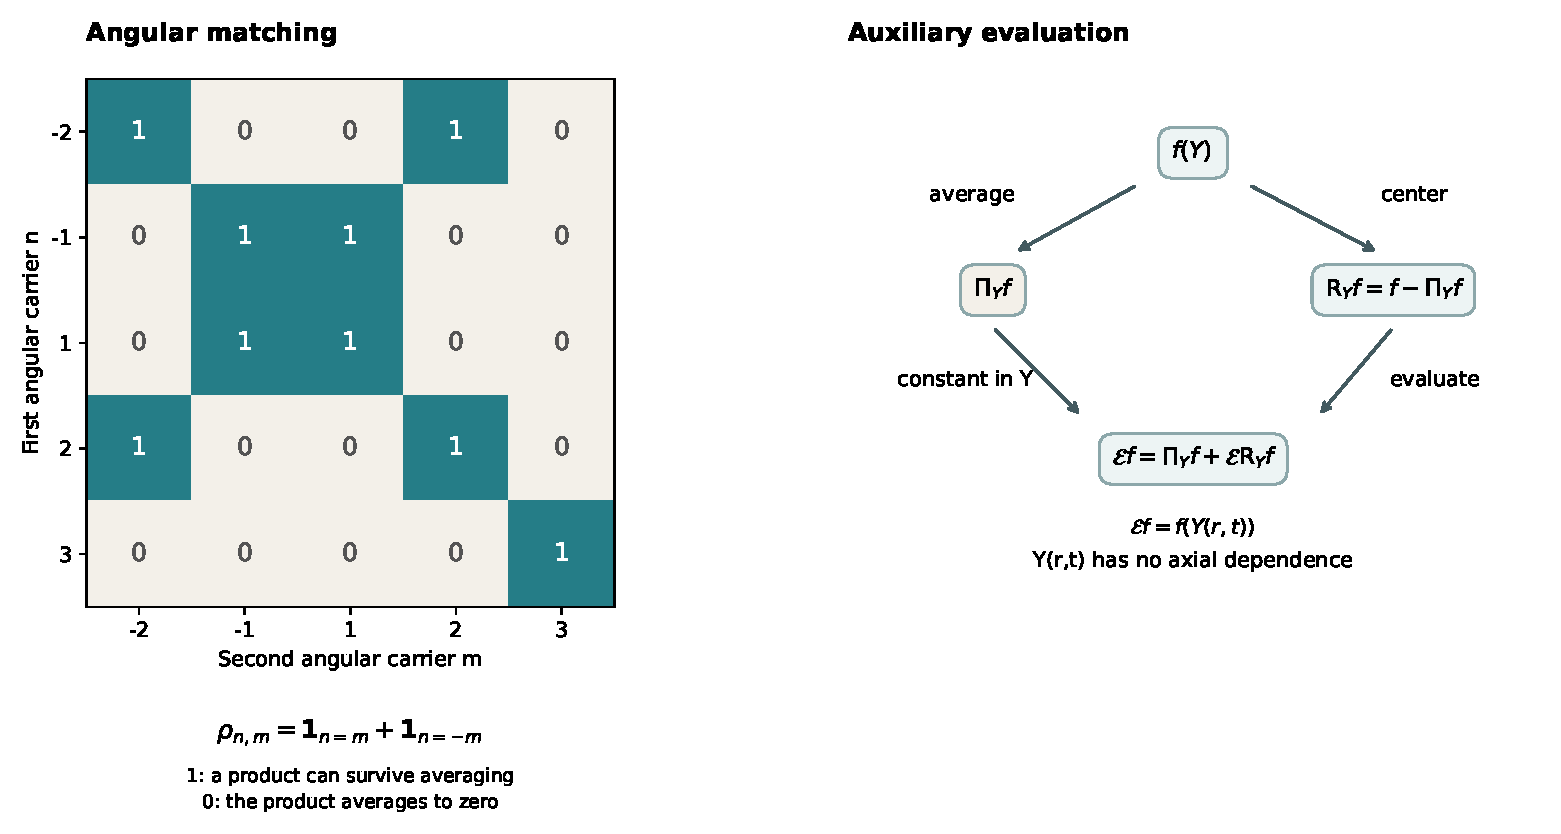
\includegraphics[width=.98\textwidth]{flux_maps.pdf}
\caption{Exact angular matching and auxiliary evaluation.
Left: the displayed finite carriers illustrate $\rho_{n,m}$;
a value one permits a signed kernel, not necessarily positive flux.
Right: evaluation retains the centered auxiliary part.
Proofs: \eqref{eflux:kernel}--\eqref{eflux:angular} and
\eqref{eflux:evaluation-identity}--\eqref{eflux:evaluation-bound}.
Source conventions: (3.7)--(3.9).
This is a diagram of exact maps, not a sampled PDE solution.
Reproducible source: \texttt{draw\_flux\_maps.py}.}
\label{eflux:figure}
\end{figure}

\section{Source and proof record}
\label{eflux:sources}
The source is OpenAI, \emph{Finite Time Blowup for Navier--Stokes}
(2026). Its \href{https://openai.com/index/navier-stokes-solution/}{official
announcement}, dated 8 September 2026, describes finite-time blowup
from zero velocity under smooth forcing, with finite energy.
The kernel, finite bounds, exponents, and reflection identities in this
addendum are proved in full above.

The TeX inspected for the averaging notation is an independent
\href{https://github.com/KokunoYumeto/openai-navier-stokes-latex/tree/5e162f34cd2d3581f890660e81fbf063509085d0}{reconstruction at commit
\texttt{5e162f34}}, specifically
\texttt{reconstruction/sections/pp013-018.tex}, lines 284--374,
including (3.7)--(3.9). It is not original author TeX.
The supplied bounded search did not locate original author TeX.
The local record preserves the full version, fetched-file hashes,
and actual reading coverage. The related archive is
\href{https://doi.org/10.5281/zenodo.22852310}{DOI 10.5281/zenodo.22852310}.
No personal attribution is inferred from an account name.

The cumulative reader retains the complete earlier physical
compact-curl moment derivation and phase map. The present addition
fills its finite evaluated-flux coefficient calculation.
Uniform bounds for an increasing family of bands and the distinct
modified sequence's terminal smooth-force extension do not follow
from the finite norms proved here.
